\chapter{Discrete Parametric Distribution Families}
\label{dispar}

The notion of a {\it parametric family} of distributions 
is a key concept that will recur throughout the book.

Consider plotting the curves $g_{a,b}(t) = (t-a)^2 + b$.  For each {\it
a} and {\it b}, we get a different parabola, as seen in this plot of
three of the curves:

% p <- ggplot(data.frame(x=c(-5,5)),aes(x))
% prb <- function(t) t^2
% prba <- function(t) (t-1)^2 
% prbb <- function(t) (t+1.5)^2 + 3
% p3 <- p + stat_function(fun = prb) + stat_function(fun = prba) +
%    stat_function(fun = prbb)
% p3 + annotate("text",x=4.8,y=27,label="a=0, b=0") +
%      annotate("text",x=-3.8,y=33,label="a=1, b=0") +
%      annotate("text",x=0.8,y=15,label="a=-1.5, b=3")

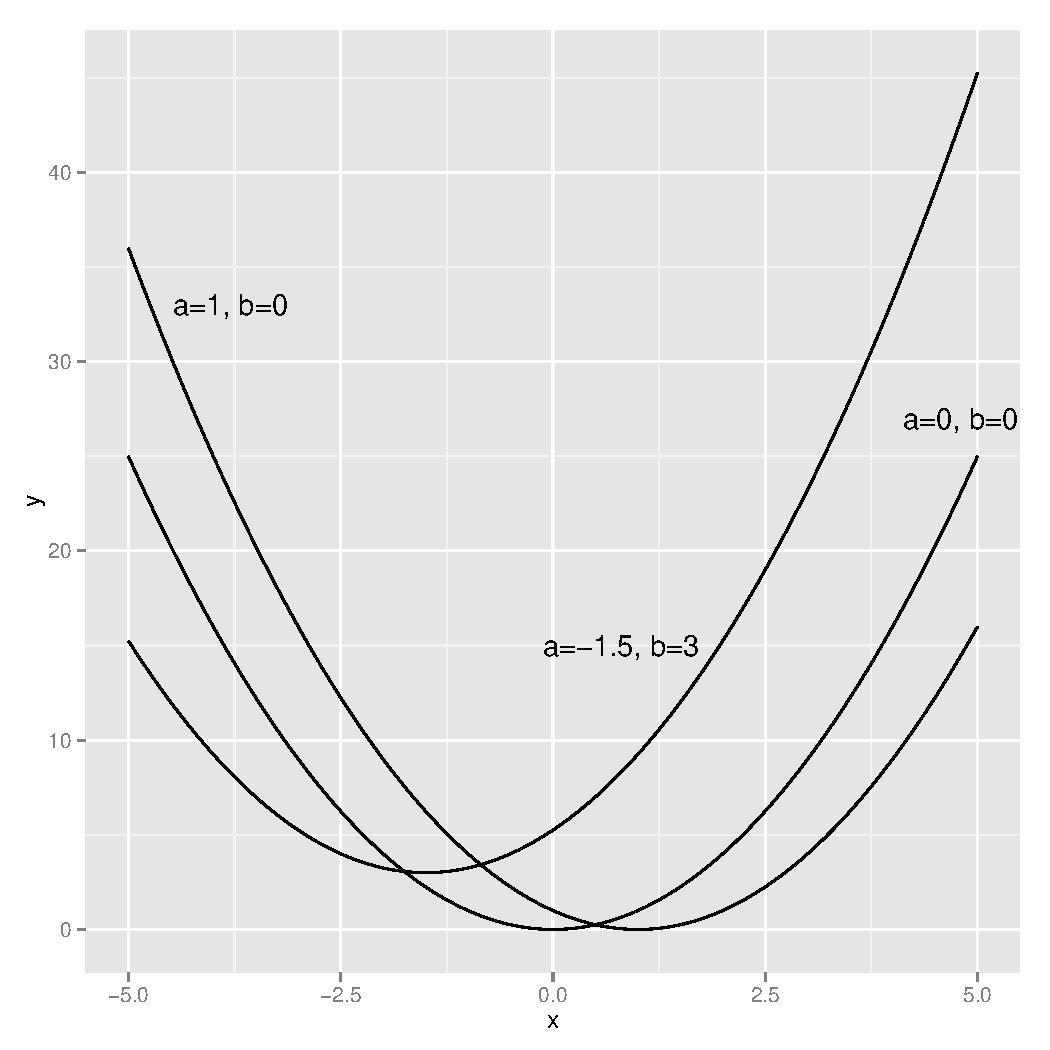
\includegraphics[width=3.5in]{Parabs.pdf}

This is a family of curves, thus a family of functions.  We say the
numbers {\it a} and {\it b} are the {\bf parameters} of the family.
Note carefully that {\it t} is not a parameter, but rather just an
argument of each function.  The point is that {\it a} and {\it b} are
indexing the curves.

\section{The Case of Importance to Us:  Parameteric Families of pmfs}

Probability mass functions are still functions.\footnote{The domains of
these functions are typically the integers, but that is irrelevant; a
function is a function.}  Thus they too can come in parametric families,
indexed by one or more parameters.  We had an example in Section
\ref{strogatz}.  Since we get a different function $p_M$ for each
different values of k and n, that was a parametric family of pmfs,
indexed by k and n.

Some parametric families of pmfs have been found to be so useful over
the years that they've been given names.  We will discuss some of those
families here.  But remember, they are famous just because they have
been found useful, i.e. that they fit real data well in various
settings.  {\bf Do not jump to the conclusion that we always ``must''
use pmfs from some family.}

\section{The Geometric Family of Distributions}
\label{geom}

To explain our first parametric family of pmfs, recall our example of
tossing a coin until we get the first head, with N denoting the number
of tosses needed.  In order for this to take k tosses, we need k-1 tails
and then a head.  Thus

\begin{equation}
p_N(k) = \large (1 - \frac{1}{2} \large )^{k-1} \cdot \frac{1}{2}, k = 1,2,...
\end{equation}

We might call getting a head a ``success,'' and refer to a tail as a
``failure.''  Of course, these words don't mean anything; we simply
refer to the outcome of interest (which of course we ourselves choose)
as ``success.''

Define M to be the number of rolls of a die needed until the number 5
shows up.  Then

\begin{equation}  
p_M(k) = \left (1 - \frac{1}{6} \right )^{k-1} \frac{1}{6}, k = 1,2,...
\end{equation}

reflecting the fact that the event \{M = k\} occurs if we get k-1 non-5s
and then a 5.  Here ``success'' is getting a 5.

The tosses of the coin and the rolls of the die are known as {\bf
Bernoulli trials}, which is a sequence of independent events.  We call
the occurrence of the event {\bf success} and the nonoccurrence {\bf
failure} (just convenient terms, not value judgments).  The associated
indicator random variable are denoted $B_i$, i = 1,2,3,...  So $B_i$ is
1 for success on the i$^{th}$ trial, 0 for failure, with success
probability p.  For instance, p is 1/2 in the coin case, and 1/6 in the
die example.  

In general, suppose the random variable W is defined to be the number 
of trials needed to get a success in a sequence of Bernoulli trials.
Then

\begin{equation}
\label{geompmf}
p_W(k) = (1-p)^{k-1} p, k = 1,2,...
\end{equation}

Note that there is a different distribution for each value of p, so we
call this a {\bf parametric family} of distributions, indexed by the
parameter p.  We say that W is {\bf geometrically distributed} with
parameter p.\footnote{Unfortunately, we have overloaded the letter {\it
p} here, using it to denote the probability mass function on the left
side, and the unrelated parameter p, our success probability on the
right side.  It's not a problem as long as you are aware of it, though.}

It should make good intuitive sense to you that

\begin{equation}
\label{eofgeom}
E(W) = \frac{1}{p}
\end{equation}

This is indeed true, which we will now derive.  First we'll need some
facts (which you should file mentally for future use as well):

{\bf Properties of Geometric Series:}

\begin{itemize}

\item [(a)] For any $t \neq 1$ and any nonnegative integers $r \leq s$,

\begin{equation}
\label{finitegeom}
\sum_{i=r}^s t^i = t^r \frac{1-t^{s-r+1}}{1-t}
\end{equation}

This is easy to derive for the case r = 0, using mathematical induction.
For the general case, just factor out $t^{r}$.

\item [(b)] For $|t| < 1$,

\begin{equation}
\label{infgeom}
\sum_{i=0}^{\infty} t^i = \frac{1}{1-t}
\end{equation}

To prove this, just take r = 0 and let $s \rightarrow \infty$ in
(\ref{finitegeom}).

\item [(c)] For $|t| < 1$,

\begin{equation}
\label{derivgeom}
\sum_{i=1}^{\infty} i t^{i-1} = \frac{1}{(1-t)^2}
\end{equation}

This is derived by applying $\frac{d}{dt}$ to
(\ref{infgeom}).\footnote{To be more careful, we should differentiate
(\ref{finitegeom}) and take limits.}

\end{itemize}

Deriving (\ref{eofgeom}) is then easy, using (\ref{derivgeom}):

\begin{eqnarray}
EW &=& \sum_{i=1}^{\infty} i (1-p)^{i-1} p \\ 
&=& p \sum_{i=1}^{\infty} i (1-p)^{i-1} \\ 
&=& p \cdot \frac{1}{[1-(1-p)]^2} \\
&=& \frac{1}{p}  \label{meangeom}
\end{eqnarray}

Using similar computations, one can show that

\begin{equation}
\label{vargeom}
Var(W) = \frac{1-p}{p^2}
\end{equation}

We can also find a closed-form expression for the quantities $P(W \leq
m)$, m = 1,2,...  (This has a formal name $F_W(m)$ , as will be seen
later in Section \ref{presentsaproblem}.)  For any positive integer m we
have

\begin{eqnarray}
F_W(m) &=& P(W \leq m) \\
&=& 1 - P(W > m) \\
&=& 1 - P(\textrm{the first m trials are all failures}) \\
&=& 1 -  (1-p)^{m}
\label{geomcdf}
\end{eqnarray}

By the way, if we were to think of an experiment involving a geometric
distribution in terms of our notebook idea, the notebook would have an
infinite number of columns, one for each $B_i$.  Within each row of the
notebook, the $B_i$ entries would be 0 until the first 1, then NA (``not
applicable'') after that.

\subsection{R Functions} 

You can simulate geometrically distributed random variables via R's {\bf
rgeom()} function.  Its first argument specifies the number of such
random variables you wish to generate, and the second is the success
probability p.

For example, if you run

\begin{Verbatim}[fontsize=\relsize{-2}]
> y <- rgeom(2,0.5)
\end{Verbatim}

then it's simulating tossing a coin until you get a head ({\bf y[1]}) and
then tossing the coin until a head again ({\bf y[2]}).  Of course, you
could simulate on your own, say using {\bf sample()} and {\bf while()},
but R makes it convenient for you.

Here's the full set of functions for a geometrically distributed random
variable X with success probability p:

\begin{itemize}

\item {\bf dgeom(i,p)}, to find $P(X = i)$

\item {\bf pgeom(i,p)}, to find $P(X \leq i)$

\item {\bf qgeom(q,p)}, to find c such that $P(X \leq c) = q$

\item {\bf rgeom(n,p)}, to generate n variates from this geometric
distribution

\end{itemize}

{\bf Important note:}  Some books define geometric distributions
slightly differently, as the number of failures before the first
success, rather than the number of trials to the first success.  The
same is true for software---both R and Python define it this way.  Thus
for example in calling {\bf dgeom()}, subtract 1 from the value used in
our definition.

For example, here is P(N = 3) for a geometric distribution under our
defintion, with p = 0.4:

\begin{lstlisting}
> dgeom(2,0.4)
[1] 0.144
> # check
> (1-0.4)^(3-1) * 0.4
[1] 0.144
\end{lstlisting}

Note that this also means one must {\it add} 1 to the result of {\bf
rgeom()}.

\subsection{Example:  a Parking Space Problem}
\label{parking}

Suppose there are 10 parking spaces per block on a certain street.  You
turn onto the street at the start of one block, and your destination is
at the start of the next block.  You take the first parking space you
encounter.  Let D denote the distance of the parking place you find from
your destination, measured in parking spaces.  Suppose each space is
open with probability 0.15, with the spaces being independent.  Find ED.

To solve this problem, you might at first think that D follows a
geometric distribution. {\bf But don't jump to conclusions!}  Actually
this is not the case; D is a somewhat complicated distance.  But clearly
D is a function of N, where the latter denotes the number of parking
spaces you see until you find an empty one---and N {\it is}
geometrically distributed.

As noted, D is a function of N: 

\begin{equation}
\label{dncases}
D = 
\begin{cases}
11-N,  & N \leq 10 \cr
N-11,  & N  > 10 \cr
\end{cases}
\end{equation}

Since D is a function of N, we can use (\ref{egofx}) with g(t) as in
(\ref{dncases}):

\begin{equation}
\label{expectdist}
ED = \sum_{i=1}^{10} (11-i) (1-0.15)^{i-1} 0.15 +
\sum_{i=11}^{\infty} (i-11) 0.85^{i-1} 0.15 
\end{equation}

This can now be evaluated using the properties of geometric series
presented above.

Alternatively, here's how we could find the result by simulation:

\begin{lstlisting}[numbers=left]
parksim <- function(nreps) {
   # do the experiment nreps times, recording the values of N
   nvals <- rgeom(nreps,0.15) + 1
   # now find the values of D
   dvals <- ifelse(nvals <= 10,11-nvals,nvals-11)
   # return ED
   mean(dvals)
}
\end{lstlisting}

Note the vectorized addition and recycling (Section
\ref{improvingsimcode}) in the line

\begin{lstlisting}
nvals <- rgeom(nreps,0.15) + 1
\end{lstlisting}

The call to {\bf ifelse()} is another instance of R's vectorization, a
vectorized if-then-else.  The first argument evaluates to a vector of
TRUE and FALSE values.  For each TRUE, the corresponding element of {\bf
dvals} will be set to the corresponding element of the vector {\bf
11-nvals} (again involving vectorized addition and recycling), and for
each false, the element of {\bf dvals} will be set to the element of
{\bf nvals-11}.

Let's find some more, first $p_N(3)$:

\begin{equation}
p_N(3) = P(N = 3) = (1-0.15)^{3-1} 0.15
\end{equation}

Next, find P(D = 1):

\begin{eqnarray}
P(D = 1) &=& P(N = 10 \textrm{ or } N = 12) \\
&=& (1-0.15)^{10-1} 0.15 + (1-0.15)^{12-1} 0.15
\end{eqnarray}

Say Joe is the one looking for the parking place.  Paul is watching from
a side street at the end of the first block (the one before the
destination), and Martha is watching from an alley situated right after
the sixth parking space in the second block.  Martha calls Paul and
reports that Joe never went past the alley, and Paul replies that he did
see Joe go past the first block.  They are interested in the probability
that Joe parked in the second space in the second block.  In
mathematical terms, what probability is that?  Make sure you understand
that it is $P(N = 12 ~|~ N > 10 \textrm{ and } N \leq 16)$.  It can be
evaluated as above.

Also:  Good news!  I found a parking place just one space away from the
destination.  Find the probability that I am parked in the same block as
the destination.

\begin{eqnarray}
P(N = 12 ~|~ N = 10 \textrm{ or } N = 12) &=&
\frac{P(N = 12)}{P(N = 10 \textrm{ or } N = 12)} \\
&=& \frac
{(1-0.15)^{11} ~ 0.15}
{(1-0.15)^{9} ~ 0.15 + (1-0.15)^{11} ~ 0.15}
\end{eqnarray}

\section{The Binomial Family of Distributions}
\label{binom}

A geometric distribution arises when we have Bernoulli trials with
parameter p, with a variable number of trials (N) but a fixed number of
successes (1).  A {\bf binomial distribution} arises when we have the
opposite---a fixed number of Bernoulli trials (n) but a variable number
of successes (say X).\footnote{Note again the custom of using capital
letters for random variables, and lower-case letters for constants.}

For example, say we toss a coin five times, and let X be the number of
heads we get.  We say that X is binomially distributed with parameters n
= 5 and p = 1/2.  Let's find P(X = 2).  There are many orders in which
that could occur, such as HHTTT, TTHHT, HTTHT and so on.  Each order has
probability $0.5^2(1-0.5)^3$, and there are $\binom{5}{2}$ orders.  Thus

\begin{equation}
P(X = 2) = \binom{5}{2} 0.5^2(1-0.5)^3 = \binom{5}{2} / 32 = 5/16 
\end{equation}

For general n and p,

\begin{equation}
p_X(k) = P(X = k) = \binom{n}{k} p^k (1-p)^{n-k}  
\end{equation}

So again we have a parametric family of distributions, in this case a
family having two parameters, n and p.

Let's write X as a sum of those 0-1 Bernoulli variables we used in the
discussion of the geometric distribution above:

\begin{equation}
X = \sum_{i=1}^{n} B_i
\end{equation}

where $B_i$ is 1 or 0, depending on whether there is success on the
$i^{th}$ trial or not.  Note again that the $B_i$ are indicator random
variables (Section \ref{indicator}),  so 

\begin{equation}
EB_i = p
\end{equation}

and 

\begin{equation}
Var(B_i) = p(1-p)
\end{equation}

Then the reader should use our earlier properties of E() and Var() in
Sections \ref{expval} and \ref{variance} to fill in the details in the
following derivations of the expected value and variance of a binomial
random variable:

\begin{equation}
\label{binmean}
EX = E(B_1+...,+B_n) = EB_1 + ... + EB_n = np
\end{equation}

and from (\ref{varsum}),

\begin{equation}
\label{binvar}
Var(X) = Var(B_1+...+B_n) = Var(B_1) + ... + Var(B_n) = np(1-p)
\end{equation}

Again, (\ref{binmean}) should make good intuitive sense to you.

\subsection{R Functions} 

Relevant functions for a binomially  distributed random variable X for k
trials and with success probability p are:

\begin{itemize}

\item {\bf dbinom(i,k,p)}, to find $P(X = i)$

\item {\bf pbinom(i,k,p)}, to find $P(X \leq i)$

\item {\bf qbinom(q,k,p)}, to find c such that $P(X \leq c) = q$ 

\item {\bf rbinom(n,k,p)}, to generate n independent values of X

\end{itemize}

Our definition above of {\bf qbinom()} is not quite tight, though.
Consider a random variable X which has a binomial distribution with n =
2 and p = 0.5。  Then

\begin{equation}
F_X(0) = 0.25, ~ F_X(1) = 0.50
\end{equation}

So if q is, say, 0.33, there is no c such that $P(X \leq c) = q$.  For
that reason, the actual definition of {\bf qbinom()} is the smallest c
satisfying $P(X \leq c) \ge q$.

\subsection{Example:  Parking Space Model}

Recall Section \ref{parking}.  Let's find the probability that there are
three open spaces in the first block.

Let M denote the number of open spaces in the first block.  This fits
the definition of binomially-distributed random variables:  We have a
fixed number (10) of independent Bernoulli trials, and we are interested
in the number of successes.  So, for instance,

\begin{equation}
p_{M}(3) = \binom{10}{3} 0.15^3 (1 - 0.15)^{10-3}
\end{equation}


\section{The Negative Binomial Family of Distributions}
\label{negbin}

Recall that a typical example of the geometric distribution family
(Section \ref{geom}) arises as N, the number of tosses of a coin needed
to get our first head.  Now generalize that, with N now being the number
of tosses needed to get our $r^{th}$ head, where r is a fixed value.
Let's find P(N = k), k = r, r+1, ...  For concreteness, look at the case
r = 3, k = 5.  In other words, we are finding the probability that it
will take us 5 tosses to accumulate 3 heads.

First note the equivalence of two events: 

\begin{equation}
\{N = 5\} = \{2 {\rm ~heads~in~the~first~} 4 {\rm ~tosses~and~head~on~the~}
5^{th} {\rm ~toss} \}
\end{equation}

That event described before the ``and'' corresponds to a binomial
probability:

\begin{equation}
P(2 {\rm ~heads~in~the~first~4~tosses}) = \binom{4}{2}
\left (\frac{1}{2} \right )^{4}
\end{equation}

Since the probability of a head on the $k^{th}$ toss is 1/2 and the
tosses are independent, we find that

\begin{equation}
P(N = 5) =  \binom{4}{2} \left (\frac{1}{2} \right )^5 = \frac{3}{16}
\end{equation}

The negative binomial distribution family, indexed by parameters r and
p, corresponds to random variables that count the number of independent
trials with success probability p needed until we get r successes.  The
pmf is

\begin{equation}
\label{negbinpmf}
p_N(k) = P(N = k) =  \binom{k-1}{r-1} (1-p)^{k-r} p^r, k = r, r+1, ...
\end{equation}

We can write

\begin{equation}
N = G_1+...+G_r
\end{equation}

where $G_i$ is the number of tosses between the successes numbers i-1
and i.  But each $G_i$ has a geometric distribution!  Since the mean of
that distribution is 1/p, we have that

\begin{equation}
E(N) = r \cdot \frac{1}{p}
\end{equation}

In fact, those r geometric variables are also independent, so we know
the variance of N is the sum of their variances:

\begin{equation}
Var(N) = r \cdot \frac{1-p}{p^2}
\end{equation} 

\subsection{R Functions}

Relevant functions for a negative binomial distributed random variable X
with success parameter p are:

\begin{itemize}

\item {\bf dnbinom(i,size=1,prob=p)}, to find $P(X = i)$

\item {\bf pnbinom(i,size=1,prob=p)}, to find $P(X <= i)$

\item {\bf qnbinom(q,sixe=1,prob=p)}, to find c such that $P(X \leq c) = q$

\item {\bf rnbinom(n,size=1,prob=p)}, to generate n independent values of X

\end{itemize}

\subsection{Example:  Backup Batteries}

A machine contains one active battery and two spares.  Each
battery has a 0.1 chance of failure each month.  Let L denote the
lifetime of the machine, i.e. the time in months until the third battery
failure.  Find P(L = 12).

The number of months until the third failure has a negative
binomial distribution, with r = 3 and p = 0.1.  Thus the answer is
obtained by (\ref{negbinpmf}), with k = 12:

\begin{equation}
P(L = 12) = \binom{11}{2} (1-0.1)^9 0.1^3
\end{equation}


\section{The Poisson Family of Distributions}
\label{poisfam}

Another famous parametric family of distributions is the set of {\bf
Poisson Distributions}.  

This family is a little different from the geometric, binomial and
negative binomial families, in the sense that in those cases there were
qualitative descriptions of the settings in which such distributions
arise.  Geometrically distributed random variables, for example occur as
the number of Bernoulli trials needed to get the first success.

By contrast, the Poisson family does not really have this kind of
qualitative description.\footnote{Some such descriptions are possible in
the Poisson case, but they are complicated and difficult to verify.} It
is merely something that people have found to be a reasonably accurate
model of actual data in many cases.  We might be interested, say, in the
number of disk drive failures in periods of a specified length of time.
If we have data on this, we might graph it, and if it looks like the pmf
form below, then we might adopt it as our model.

The pmf is

\begin{equation}
\label{poispmf}
P(X = k) = \frac{e^{- \lambda} \lambda^k}{k!}, k = 0,1,2,...
\end{equation}

It turns out that

\begin{equation}
EX = \lambda
\end{equation}

\begin{equation}
Var(X) = \lambda
\end{equation}

The derivations of these facts are similar to those for the geometric
family in Section \ref{geom}.  One starts with the Maclaurin series
expansion for $e^t$:

\begin{equation}
e^t = \sum_{i=0}^{\infty} \frac{t^i}{i!}
\end{equation}

and finds its derivative with respect to t, and so on.  The details are
left to the reader.

\label{bankex}
The Poisson family is very often used to model count data.  For example,
if you go to a certain bank every day and count the number of customers
who arrive between 11:00 and 11:15 a.m., you will probably find that that
distribution is well approximated by a Poisson distribution for some
$\lambda$.

There is a lot more to the Poisson story than we see in this short
section.  We'll return to this distribution family in Section
\ref{connpoi}. 

\subsection{R Functions}

Relevant functions for a Poisson distributed random variable X
with parameter lambda are:

\begin{itemize}

\item {\bf dpois(i,lambda)}, to find $P(X = i)$

\item {\bf ppois(i,lambda)}, to find $P(X \leq i)$

\item {\bf qpois(q,lambda)}, to find c such that $P(X \leq c) = q$

\item {\bf rpois(n,lambda)}, to generate n independent values of X

\end{itemize}

\subsection{Example: Broken Rod}

Recall the example of a broken glass rod in Section \ref{brokenrod}.
Suppose now that the number of breaks is random, not just the break
points.  A reasonable model to try would be Poisson.  However, 
the latter's support starts at 0, and we cannot have 0 pieces,
so we need to model the number of pieces minus 1 (the number of break
points) as Poisson.

The code is similar to that in Section \ref{brokenrod}, but we must
first generate the number of break points:

\begin{lstlisting}
minpiecepois <- function(lambda) {
   nbreaks <- rpois(1,lambda)
   breakpts <- sort(runif(nbreaks))
   lengths <- diff(c(0,breakpts,1))
   min(lengths)
}

bkrodpois <- function(nreps,lambda,q) {
   minpieces <- replicate(nreps,minpiecepois(lambda))
   mean(minpieces < q) 
}

> bkrodpois(10000,5,0.02)  
[1] 0.4655
\end{lstlisting}

Note that in each call to {\bf minpiecepois()}, there will be a
different number of breakpoints.

\section{The Power Law Family of Distributions}

This family has attracted quite a bit of attention in recent years, due
to its use in random graph models.

\subsection{The Model}

Here

\begin{equation}
p_X(k) = c k^{-\gamma}, ~ k = 1,2,3,...
\end{equation}

It is required that $\gamma > 1$, as otherwise the sum of probabilities
will be infinite.  For $\gamma$ satisfying that condition, the value c
is chosen so that that sum is 1.0:

\begin{equation}
1.0 = \sum_{k=1}^{\infty} c k^{-\gamma} \approx
c \int_1^{\infty} k^{-\gamma} ~ dk = c/(\gamma - 1)
\end{equation}

so $c \approx \gamma -1$.

Here again we have a parametric family of distributions, indexed by the
parameter $\gamma$.

The power law family is an old-fashioned model (an old-fashioned term
for {\it distribution} is {\it law}), but  there has been a resurgence
of interest in it in recent years.  Analysts have found that many types
of social networks in the real world exhibit approximately power law
behavior in their degree distributions.

For instance, in a famous study of the Web (A. Barabasi and R. Albert,
Emergence of Scaling in Random Networks, {\it Science}, 1999, 509-512),
degree distribution on the Web (a directed graph, with incoming links
being the ones of interest here) it was found that the number of links
leading to a Web page has an approximate power law distribution with
$\gamma =2.1$.  The number of links leading out of a Web page was found
to be approximately power-law distributed, with $\gamma = 2.7$.

Much of the interest in power laws stems from their {\bf fat tails}, a
term meaning that values far from the mean are more likely under a power
law than they would be under a normal distribution with the same mean.
In recent popular literature, values far from the mean have often been
called {\bf black swans}.  The financial crash of 2008, for example, is
blamed by some on the ignorance by {\bf quants} (people who develop
probabilistic models for guiding investment) in underestimating the
probabilities of values far from the mean.

Some examples of real data that are, or are not, fit well by power law
models are given in the paper {\it Power-Law Distributions in Empirical
Data}, by A. Clauset, C. Shalizi and M. Newman, at
\url{http://arxiv.org/abs/0706.1062}.  Methods for estimating the
parameter $\gamma$ are discussed and evaluated.

A variant of the power law model is the {\bf power law with exponential
cutoff}, which essentially consists of a blend of the power law and a
geometric distribution.  Here

\begin{equation}
p_X(k) = c k^{-\gamma} q^k
\end{equation}

This now is a two-parameter family, the parameters being $\gamma$ and q.
Again c is chosen so that the pmf sums to 1.0.

This model is said to work better than a pure power law for some types
of data.  Note, though, that this version does not really have the fat
tail property, as the tail decays exponentially now.

\subsection{Further Reading}

There is nice paper on fitting (or not fitting) power law models:

Power-Law Distributions in Empirical Data, {\it SIAM Review}, A.
Clauset, C.R. Shalizi, and M.E.J. Newman, 51(4), 661-703, 2009.

\section{Recognizing Some Parametric Distributions When You See Them}

Three of the discrete distribution families we've considered here arise
in settings with very definite structure, all dealing with independent
trials:

\begin{itemize}

\item the binomial family gives the distribution of the number of
successes in a fixed number of trials

\item the geometric family gives the distribution of the number of
trials needed to obtain the first success

\item the negative binomial family gives the distribution of the number of
trials needed to obtain the k$^{th}$ success

\end{itemize}

Such situations arise often, hence the fame of these distribution
families.

By contrast, the Poisson and power law distributions have no underlying
structure.  They are famous for a different reason, that it has been
found empirically that they provide a good fit to many real data sets.

In other words, the Poisson and power law distributions are typically
fit to data, in an attempt to find a good model, whereas in the binomial,
geometric and negative binomial cases, the fundamental nature of the
setting implies one of those distributions.

{\bf You should make a strong effort to get to the point at which you
automatically recognize such settings when your encounter them}.

\section{Example:  a Coin Game}
\label{coingame}

{\it Life is unfair}---former President Jimmie Carter

\bigskip

Consider a game played by Jack and Jill. Each of them tosses a coin many
times, but Jack gets a head start of two tosses. So by the time Jack has
had, for instance, 8 tosses, Jill has had only 6; when Jack tosses for
the 15$^{th}$ time, Jill has her 13$^{th}$ toss; etc.

Let $X_k$ denote the number of heads Jack has gotten through his
k$^{th}$ toss, and let $Y_k$ be the head count for Jill at that same
time, i.e.  among only k-2 tosses for her. (So, $Y_1 = Y_2 = 0$.)
Let's find the probability that Jill is winning after the 6$^{th}$
toss, i.e. $P(Y_6 > X_6)$.

Your first reaction might be, ``Aha, binomial distribution!''  You would
be on the right track, but the problem is that you would not be thinking
precisely enough.  Just WHAT has a binomial distribution?  The answer is
that both $X_6$ and $Y_6$ have binomial distributions, both with p =
0.5, but n = 6 for $X_6$ while n = 4 for $Y_6$.

Now, as usual, ask the famous question, ``How can it happen?''  How can
it happen that  $Y_6 > X_6$?  Well, we could have, for example, $Y_6 = 3$
and $X_6 = 1$, as well as many other possibilities.  Let's write it
mathematically:

\begin{equation}
\label{ygx}
P(Y_6 > X_6) = \sum_{i=1}^4 \sum_{j=0}^{i-1} P(Y_6 = i \textrm{ and } X_6 = j)
\end{equation}

Make SURE your understand this equation.

Now, to evaluate $P(Y_6 = i \textrm{ and } X_6 = j)$, we see the ``and''
so we ask whether $Y_6$ and $X_6$ are independent.  They in fact are;
Jill's coin tosses certainly don't affect Jack's.  So,

\begin{equation}
P(Y_6 = i \textrm{ and } X_6 = j) =
P(Y_6 = i) \cdot P(X_6 = j)
\end{equation}

It is at this point that we finally use the fact that $X_6$ and $Y_6$
have binomial distributions.  We have

\begin{equation}
\label{y6}
P(Y_6 = i) = \binom{4}{i} 0.5^i (1-0.5)^{4-i}  
\end{equation}

and

\begin{equation}
\label{x6}
P(X_6 = j) = \binom{6}{j} 0.5^j (1-0.5)^{6-j}  
\end{equation}

We would then substitute (\ref{y6}) and (\ref{x6}) in (\ref{ygx}).  We
could then evaluate it by hand, but it would be more convenient to use
R's {\bf dbinom()} function:

\begin{Verbatim}[fontsize=\relsize{-2},numbers=left]
prob <- 0
for (i in 1:4)
   for (j in 0:(i-1))
      prob <- prob + dbinom(i,4,0.5) * dbinom(j,6,0.5)
prob
\end{Verbatim}

We get an answer of about 0.17.  If Jack and Jill were to play this game
repeatedly, stopping each time after the 6$^{th}$ toss, then Jill
would win about 17\% of the time.

\section{Example:  Tossing a Set of Four Coins}

Consider a game in which we have a set of four coins.  We keep tossing
the set of four until we have a situation in which exactly two of them
come up heads.  Let N denote the number of times we must toss the set of
four coins.

For instance, on the first toss of the set of four, the outcome might be
HTHH.  The second might be TTTH, and the third could be THHT.  In the
situation, N = 3.

Let's find P(N = 5).  Here we recognize that N has a geometric
distribution, with ``success'' defined as getting two heads in our set
of four coins.  What value does the parameter p have here?  

Well, p is P(X = 2), where X is the number of heads we get from a toss
of the set of four coins.  We recognize that X is binomial!  Thus

\begin{equation}
p = \binom{4}{2} 0.5^4 = \frac{3}{8}
\end{equation}

Thus using the fact that N has a geometric distribution,

\begin{equation}
P(N = 5) = (1-p)^4 p = 0.057
\end{equation}

\section{Example:  the ALOHA Example Again}
\label{alohaagain}

As an illustration of how commonly these parametric families arise,
let's again look at the ALOHA example.  Consider the general case, with
transmission probability p, message creation probability q, and m
network nodes.  We will not restrict our observation to just two epochs.

Suppose $X_i = m$, i.e. at the end of epoch i all nodes have a message
to send.  Then the number which attempt to send during epoch i+1 will be
binomially distributed, with parameters m and p.\footnote{Note that
this is a conditional distribution, given $X_i = m$.}  For instance, the
probability that there is a successful transmission is equal to the
probability that exactly one of the m nodes attempts to send,

\begin{equation}
\label{onesends}
\binom{m}{1} p (1-p)^{m-1} = mp(1-p)^{m-1}
\end{equation}

Now in that same setting, $X_i = m$, let K be the number of epochs it
will take before some message actually gets through.  In other words, we
will have $X_i = m$, $X_{i+1} = m$, $X_{i+2} = m$,...  but finally
$X_{i+K-1} = m-1$.  Then K will be geometrically distributed, with
success probability equal to (\ref{onesends}).

There is no Poisson distribution in this example, but it is central to
the analysis of Ethernet, and almost any other network.  We will discuss
this at various points in later chapters.

\section{Example:  the Bus Ridership Problem Again}

Recall the bus ridership example of Section \ref{busridership}.  Let's
calculate some expected values, for instance $E(B_1)$:

\begin{equation}
\label{eb1}
E(B_1) =
0 \cdot P(B_1 = 0) +
1 \cdot P(B_1 = 1) +
2 \cdot P(B_1 = 2) = 0.4 + 2 \cdot 0.1
\end{equation}

Now suppose the company charges \$3 for passengers who board at the
first stop, but charges \$2 for those who join at the second stop.  (The
latter passengers get a possibly shorter ride, thus pay less.) So, the
total revenue from the first two stops is $T = 3 B_1 + 2 B_2$.  Let's
find E(T).  We'd write

\begin{equation}
E(T) = 3 E(B_1) + 2 E(B_2)
\end{equation}

making use of (\ref{aubv}).  We'd then compute the terms as in
\ref{eb1}.

Suppose the bus driver has the habit of exclaiming, ``What?  No new
passengers?!'' every time he comes to a stop at which $B_i = 0$.  Let N
denote the number of the stop (1,2,...) at which this first occurs.
Find P(N = 3):

N has a geometric distribution, with p equal to the probability that
there 0 new passengers at a stop, i.e. 0.5.  Thus $p_N(3) = (1-0.5)^2 0.5$,
by (\ref{geompmf}).

Let S denote the number of stops, out of the first 6, at which 2 new
passengers board.  For example, S would be 3 if $B_1 = 2$, $B_2 = 2$,
$B_3 = 0$, $B_4 = 1$, $B_5 = 0$, and $B_6 = 2$.  Find $p_S(4)$:

S has a binomial distribution, with n = 6 and p = probability
of 2 new passengers at a stop = 0.1.  Then

\begin{equation}
p_S(4) = \binom{6}{4} 0.1^4 (1-0.1)^{6-4}
\end{equation}

By the way, we can exploit our knowledge of binomial distributions to
simplify the simulation code in Section \ref{busridershipsim}.  The
lines

\begin{lstlisting}
for (k in 1:passengers)
   if (runif(1) < 0.2)
      passengers <- passengers - 1
\end{lstlisting}

simulate finding that number of passengers that alight at that stop.
But that number is binomially distributed, so the above code can be
compactified (and speeded up in execution) as

\begin{lstlisting}
passengers <- passengers - rbinom(1,passengers,0.2)
\end{lstlisting}

\section{Example:  Flipping Coins with Bonuses}
\label{bonusflip}

A game involves flipping a coin k times.  Each time you get a head, you
get a bonus flip, not counted among the k.  (But if you get a head from
a bonus flip, that does not give you its own bonus flip.) Let X denote
the number of heads you get among all flips, bonus or not.  Let's find
the distribution of X.

As with the parking space example above, we should be careful not to
come to hasty conclusions.  The situation here ``sounds'' binomial, but
X, based on a variable number of trials, doesn't fit the definition of
binomial.

But let Y denote the number of heads you obtain through
nonbonus flips.  Y then has a binomial distribution with parameters k
and 0.5.  To find the distribution of X, we'll condition on Y.  

We will as usual ask, ``How can it happen?'', but we need to take extra
care in forming our sums, recognizing constraints on Y:

\begin{itemize}

\item $Y \geq X/2$

\item $Y \leq X$

\item $Y \leq k$

\end{itemize}

Keeping those points in mind, we have

\begin{eqnarray}
p_X(m) &=& P(X = m) \\ 
&=& \sum_{i=\textrm{ceil}(m/2)}^{\min(m,k)} 
   P(X = m \textrm{ and } Y = i) \\
&=& \sum_{i=\textrm{ceil}(m/2)}^{\min(m,k)} 
   P(X = m | Y = i) ~ P(Y = i)\\
&=& \sum_{i=\textrm{ceil}(m/2)}^{\min(m,k)} 
   \binom{i}{m-i} 0.5^i \binom{k}{i} 0.5^k \\
&=& 0.5^k \sum_{i=\textrm{ceil}(m/2)}^{\min(m,k)} 
   \frac{k!}{(m-i)!(2i-m)!(k-i)!} 0.5^i
\end{eqnarray}

There doesn't seem to be much further simplification possible here.

\section{Example:  Analysis of Social Networks}
\label{socnets}

Let's continue our earlier discussion from Section \ref{strogatz}.

One of the earliest---and now the simplest---models of social networks
is due to Erd\"{o}s and Renyi.  Say we have n people (or n Web sites,
etc.), with $\binom{n}{2}$ potential links between pairs.  (We are
assuming an undirected graph here.)  In this model, each potential link
is an actual link with probability p, and a nonlink with probability
1-p, with all the potential links being independent.

Recall the notion of degree distribution from Section \ref{strogatz}.
Clearly the degree distribution $D_i$ here for a single node i is
binomial with parameters n-1 and p.  

But consider k nodes, say 1 through k, among the n total nodes, and let
T denote the number of links involving these nodes.  Let's find the
distribution of T.  That distribution is again binomial, but the number
of trials must be carefully calculated.  We cannot simply say that,
since each of the k vertices can have as many as n-1 links, there are
k(n-1) potential links, because there is overlap; two nodes among the k
have a potential link with each other, but we can't count it twice.  So,
let's reason this out.

Say n = 9 and k = 4.  Among the four special nodes, there are $\binom{4}{2}
= 6$ potential links, each on or off with probability p, independently.
Also each of the four special nodes has $9 - 4 = 5$ potential links with
the ``outside world,'' i.e.\ the five non-special nodes.  So there are
$4 \times 5 = 20$ potential links here, for a total of 26.

So, the distribution of T is binomial with

\begin{equation}
\label{knk2}
k (n-k) + \binom{k}{2}
\end{equation}

trials and success probability p.

\section{Multivariate Distributions}
\label{minimul}

(I am borrowing some material here from Section \ref{marblepmf}, for
instructors or readers who skip Chapter \ref{mul}.  It is important to
know that multivariate distributions exist, even if one doesn't know the
details.)

Recall that for a single discrete random variable X, the distribution of
X was defined to be a list of all the values of X, together with the
probabilities of those values.  The same is done for a pair (or more
than a pair) of discrete random variables U and V.

Suppose we have a bag containing two yellow marbles, three blue ones and
four green ones.  We choose four marbles from the bag at random,
without replacement.  Let Y and B denote the number of yellow and blue
marbles that we get.  Then define the {\it two-dimensional} pmf of Y and
B to be

\begin{equation}
p_{Y,B}(i,j) = P(Y = i \textrm{ and } B = j) = 
\frac
{
\binom{2}{i}
\binom{3}{j}
\binom{4}{4-i-j}
}
{\binom{9}{4}}
\end{equation}

Here is a table displaying all the values of P(Y = i and B = j):

\begin{tabular}{|r|r|r|r|r|r|}
\hline
i $\downarrow$, j $\rightarrow$ & 0 & 1 & 2 & 3 \\ \hline
0 & 0.008 & 0.095 & 0.143 & 0.032 \\ \hline
1 & 0.063 & 0.286 & 0.190 & 0.016 \\ \hline
2 & 0.048 & 0.095 & 0.024 & 0.000 \\ \hline
\end{tabular}

So this table is the distribution of the pair (Y,B).

Recall further that in the discrete case, we introduced a symbolic
notation for the distribution of a random variable X, defined as
$p_X(i) = P(X = i)$, where i ranged over the support of X.
We do the same thing for a pair of random variables:

\begin{definition}
For discrete random variables U and V, their
probability mass function is defined to be

\begin{equation}
p_{U,V}(i,j) = P(U = i \textrm{ and } V = j)
\end{equation}

where (i,j) ranges over all values taken on by (U,V).
Higher-dimensional pmfs are defined similarly, e.g.

\begin{equation}
p_{U,V,W}(i,j,k) = P(U = i \textrm{ and } V = j \textrm{ and } W = k)
\end{equation}
\end{definition}

So in our marble example above, $p_{Y,B}(1,2) = 0.048$, $p_{Y,B}(2,0) =
0.012$ and so on.

\section{Iterated Expectations}
\label{iterexp}

This section has an abstract title, but the contents are quite useful.

\subsection{Conditional Distributions}

Just as we can define bivariate pmfs, we can also speak of conditional
pmfs.  Suppose we have random variables U and V.  

In our bus ridership example, for instance, we can talk about

\begin{equation}
\label{el2b1}
E(L_2 ~|~ B_1 = 0) 
\end{equation}

In notebook terms, think of many replications of watching the bus during
times 1 and 2.  Then (\ref{el2b1}) is defined to be the long-run average
of values in the $L_2$ column, {\bf among those rows} in which the $B_1$
column is 0.  (And by the way, make sure you understand why
(\ref{el2b1}) works out to be 0.6.)

\subsection{The Theorem}

The key relation says, in essence,

\begin{quote}
The overall mean of V is a weighted average of the conditional means of
V given U.  The weights are the pmf of U.
\end{quote}

Note again that $E(V ~|~ U = c)$ is defined in ``notebook'' terms as the
long-run average of V, {\it among those lines in which U = c}.

Here is the formal version:

Suppose we have random variables U and V, with U discrete and with V
having  an expected value.  Then

\begin{equation}
\label{adamsdiscrete}
E(V) = \sum_c P(U = c) ~ E(V ~|~ U = c) 
\end{equation}

where c ranges through the support of U.

In spite of its intimidating form, (\ref{adamsdiscrete}) makes good
intuitive sense, as follows:  Suppose we want to find the average height
of all students at a university.  Each department measures the heights
of its majors, then reports the mean height among them.  Then
(\ref{adamsdiscrete}) says that to get the overall mean in the entire
school, we should take a {\it weighted} average of all the
within-department means, with the weights being the proportions of each
department's student numbers among the entire school.  Clearly, we would
not want to take an unweighted average, as that would count tiny
departments just as much as large majors.

Here is the derivation (reader:  supply the reasons!).

\begin{eqnarray}
EV &=& \sum_{d} d ~ P(V = d) \\ 
   &=& \sum_{d} d ~ \sum_{c} P(U = c \textrm{ and } V = d) \\ 
   &=& \sum_{d} d ~ \sum_{c} P(U = c) ~ P(V = d ~|~ U = c) \\ 
   &=& \sum_{d} \sum_{c} d ~P(U = c) ~ P(V = d ~|~ U = c) \\ 
   &=& \sum_{c} \sum_{d} d ~P(U = c) ~ P(V = d ~|~ U = c) \\ 
   &=& \sum_{c} P(U = c) \sum_{d} d ~ P(V = d ~|~ U = c) \\ 
   &=& \sum_c P(U = c) ~ E(V ~|~ U = c) 
\end{eqnarray}

\subsection{Example:  Coin and Die Game}

You roll a die until it comes up 5, taking M rolls to do so.  You then
toss a coin M times, winning one dollar for each head.  Find the
expected winnings, EW.

Solution:  Given M = k, the number of heads has a binomial distribution
with n = k and p = 0.5.  So

\begin{equation}
E(W | M = k) = 0.5 k.
\end{equation}

So, from (\ref{adamsdiscrete}), we have

\begin{equation}
EW = \sum_{k=1}^\infty P(M = k) ~ 0.5 k 
= 0.5 \sum_{k=1}^\infty P(M = k) k
= 0.5 ~ EM
\end{equation}

from (\ref{a}).  And from (\ref{eofgeom}), we know EM = 6.  So, EW = 3.

\subsection{Example: Flipping Coins with Bonuses}

Recall the example in Section \ref{bonusflip}.  The principle of
iterated expectation can easily get us $EX$:

\begin{eqnarray}
EX &=& \sum_{i=1}^k P(Y = i) ~ E(X | Y = i) \\
   &=& \sum_{i=1}^k P(Y = i) ~ (i + 0.5i) \\
   &=& E(1.5Y) \\
   &=& 1.5 \cdot k/2 \\
   &=& 0.75k
\end{eqnarray}

To understand that second equality, note that if $Y = i$, $X$ will
already include those $i$ heads, the nonbonus heads, and since there
will be $i$ bonus flips, the expected value of the number of bonus heads
will be $0.5 i$.  The third equality uses (\ref{egofx}) (in a reverse
manner).

\startproblemset

\oneproblem
Consider a game in which one rolls a single die until one accumulates a
total of at least four dots. Let $X$ denote the number of rolls needed.
Find $P(X \leq 2)$ and $E(X)$.

\oneproblem
Recall the committee example in Section \ref{combex}.  Suppose now,
though, that the selection protocol is that there must be at least one
man and at least one woman on the committee.  Find $E(D)$ and $Var(D)$.

\oneproblem
Suppose a bit stream is subject to errors, with each bit having
probability p of error, and with the bits being independent. Consider a
set of four particular bits. Let X denote the number of erroneous bits
among those four.

\begin{itemize}

\item [(a)] Find P(X = 2) and EX.

\item [(b)] What famous parametric family of distributions does the
distribution of X belong to?

\item [(c)] Let Y denote the maximum number of consecutive erroneous bits.
Find P(Y = 2) and Var(Y). 

\end{itemize}

\oneproblem
Derive (\ref{vargeom}).

\oneproblem
Finish the computation in (\ref{expectdist}).

\oneproblem
Derive the facts that for a Poisson-distributed random variable X with
parameter $\lambda$, $EX = Var(X) = \lambda$.  Use the hints in Section
\ref{poisfam}.

\oneproblem
A civil engineer is collecting data on a certain road.  She needs to
have data on 25 trucks, and 10 percent of the vehicles on that road are
trucks.  State the famous parametric family that is relevant here, and
find the probability that she will need to wait for more than
200 vehicles to pass before she gets the needed data.

\oneproblem
In the ALOHA example:

\begin{itemize}

\item [(a)] Find $E(X_1)$ and $Var(X_1)$, for the case p = 0.4, q = 0.8.
You are welcome to use quantities already computed in the text, e.g.
$P(X_1 = 1) = 0.48$, but be sure to cite equation numbers.

\item [(b)] Find P(collision during epoch 1) for general p, q.

\end{itemize}

\oneproblem
Our experiment is to toss a nickel until we get a head, taking
X rolls, and then toss a dime until we get a head, taking Y tosses.
Find:

\begin{itemize}

\item [(a)] Var(X+Y).

\item [(b)] Long-run average in a ``notebook'' column labeled $X^2$.

\end{itemize}

\oneproblem
Consider the game in Section \ref{coingame}.  Find $E(Z)$ and $Var(Z)$,
where $Z = Y_6 - X_6$.

\oneproblem
Say we choose six cards from a standard deck, one at a time WITHOUT
replacement.  Let $N$ be the number of kings we get.  Does $N$ have a
binomial distribution?  Choose one: (i)  Yes.  (ii) No, since trials are
not independent.  (iii) No, since the probability of success is not
constant from trial to trial.  (iv) No, since the number of trials is not
fixed.  (v) (ii) and (iii).  (iv) (ii) and (iv).  (vii) (iii) and (iv).  

\oneproblem
Suppose we have n independent trials, with the probability
of success on the i$^{th}$ trial being $p_i$.  Let $X$ = the number of
successes.  Use the fact that ``the variance of the sum is the sum of
the variance'' for independent random variables to derive $Var(X)$.

\oneproblem
Prove Equation (\ref{varuformula}).

\oneproblem
Show that if $X$ is a nonnegative-integer valued random variable, then

\begin{equation}
EX = \sum_{i=1}^{\infty} P(X \geq i)
\end{equation}

Hint:  Write $i = \sum_{j=1}^i 1$, and when you see an iterated sum,
reverse the order of summation.

\oneproblem
Suppose we toss a fair coin n times, resulting in $X$ heads.  Show that
the term {\it expected value} is a misnomer, by showing that

\begin{equation}
\lim_{n \rightarrow \infty} P(X = n/2) = 0
\end{equation}

Use Stirling's approximation, 

\begin{equation}
k! \approx \sqrt{2 \pi k} \left ( \frac{k}{e} \right )^k
\end{equation}

\oneproblem
Suppose X and Y are independent random variables with standard
deviations 3 and 4, respectively.

\begin{itemize}

\item [(a)] Find Var(X+Y).

\item [(b)] Find Var(2X+Y).

\end{itemize}

\oneproblem
Fill in the blanks in the following simulation, which finds
the approximate variance of N, the number of rolls of a die needed to
get the face having just one dot.

\begin{Verbatim}[fontsize=\relsize{-2}]
onesixth <- 1/6
sumn <- 0
sumn2 <- 0
for (i in 1:10000) {
   n <- 0
   while(TRUE) {
      ________________________________________
      if (______________________________ < onesixth) break
   }
   sumn <- sumn + n
   sumn2 <- sumn2 + n^2
}
approxvarn <- ____________________________________________
cat("the approx. value of Var(N) is ",approxvarn,"\n")
\end{Verbatim}

\oneproblem
Let X be the total number of dots we get if we roll three
dice.  Find an upper bound for $P(X \geq 15)$, using our course
materials.

\oneproblem
Suppose X and Y are independent random variables, and let Z = XY. Show
that $Var(Z) = E(X^2)   E(Y^2) - [E(X)]^2   [E(Y)]^2$. 

\oneproblem
This problem involves a very simple model of the Web. (Far more complex
ones exist.)

Suppose we have n Web sites. For each pair of sites i and j, $i \neq j$,
there is a link from site i to site j with probability p, and no link
(in that direction) with probability 1-p. Let $N_i$ denote the number of
sites that site i is linked to; note that $N_i$ can range from 0 to n-1.
Also, let $M_{ij}$ denote the number of outgoing links that sites i and
j have in common, not counting the one between them, if any. Assume that
each site forms its outgoing links independently of the others.

Say n = 10, p = 0.2. Find the following:

\begin{itemize}

\item [(a)] $P(N_1 = 3)$

\item [(b)] $P(N_1 = 3 \textrm{ and } N_2 = 2)$

\item [(c)] $Var(N_1)$

\item [(d)] $Var(N_1 + N_2)$

\item [(e)] $P(M_{12} = 4)$

\end{itemize}

Note: There are some good shortcuts in some of these problems, making
the work much easier. But you must JUSTIFY your work.

\oneproblem
Let X denote the number of heads we get by tossing a coin 50 times.
Consider Chebychev's Inequality for the case of 2 standard deviations.
Compare the upper bound given by the inequality to the exact probability.

\oneproblem
Suppose the number N of cars arriving during a given time period at a
toll booth has a Poisson distribution with parameter $\lambda$. Each 
car has a probability p of being in a car pool. Let M be the number of
car-pool cars that arrive in the given period. Show that M also has a Poisson   
distribution, with parameter $p \lambda$. (Hint: Use the Maclaurin series for   
$e^x$.) 

\oneproblem
Consider a three-sided die, as on page \pageref{threesideddiepage}.  Let
X denote the number of dots obtained in one roll.

\begin{itemize}

   \item [(a)] (10) State the value of $p_X(2)$.

   \item [(b)] (10) Find EX and Var(X).

   \item [(c)] (15) Suppose you win \$2 for each dot.  Find EW,
   where W is the amount you win.

\end{itemize}

\oneproblem
Consider the parking space problem in Section \ref{parking}.  Find
Var(M), where M is the number of empty spaces in the first block, and
Var(D).

\oneproblem
Suppose X and Y are independent, with variances 1 and 2,
respectively.  Find the value of c that minimizes Var[cX + (1-c)Y].

\oneproblem
In the cards example in Section \ref{hearts}, let H denote the number of
hearts. Find EH and Var(H).

\oneproblem
In the bank example in Section \ref{bankex}, suppose you observe the
bank for n days. Let X denote the number of days in which at least 2 
customers entered during the 11:00-11:15 observation period. Find P(X = k).

\oneproblem
Find $E(X^3)$, where X has a geometric distribution with parameter p.

\oneproblem
Supppose we have a nonnegative random variable X, and define a new
random variable Y, which is equal to X if X $>$ 8 and equal to 0
otherwise.  Assume X takes on only a finite number of values (just a
mathematical nicety, not really an issue).  Which one of the following
is true:

\begin{itemize}

\item [(i)] $EY \leq EX$.

\item [(ii)] $EY \geq EX$.

\item [(iii)] Either of $EY$ and $EX$ could be larger than the other,
depending on the situation.

\item [(iv)] $EY$ is undefined.

\end{itemize}

\oneproblem
Say we roll two dice, a blue one and a yellow one.  Let B
and Y denote the number of dots we get, respectively, and write S = B +
Y.  Now let G denote the indicator random variable for the event S = 2.  
Find E(G).

% \oneproblem Suppose $I_1, I_2 \textrm{ and } I_3$ are independent
% indicator random variables, with $P(I_j = 1) = p_j$, j = 1,2,3.  Find
% the following in terms of the $p_j$, writing your derivation with
% reasons in the form of mailing tube numbers. 

\oneproblem Consider the ALOHA example, Section \ref{alohaagain} .
Write a call to the built-in R function {\bf dbinom()} to evaluate
(\ref{onesends}) for general m and p.

\oneproblem Consider the bus ridership example, Section
\ref{busridership}.  Suppose upon arrival to a certain stop, there are 2
passengers.  Let A denote the number of them who choose to alight at
that stop.

\begin{itemize}

\item [(a)] State the parametric family that the distribution of A
belongs to.

\item [(b)] Find $p_A(1)$ and $F_A(1)$, writing each answer in
decimal expression form e.g. $12^8 \cdot 0.32 + 0.3333$.

\end{itemize}

\oneproblem
Suppose you have a large disk farm, so heavily used that the lifetimes L
are measured in months. They come from two different factories, in
proportions q and 1-q. The disks from factory i have geometrically
distributed lifetime with parameter $p_i$, i = 1,2. Find Var(L) in terms of
q and the $p_i$. 

\oneproblem
Show how to eliminate the inner loop in the code at the end of Section
\ref{coingame}.
